\subsection{Mercury}
\label{chap:related:mercury}
In Mercury \cite{Bharambe2004Mercury} gibt es eine Menge von Attributen, die ihrerseits einen definierten Wertebereich haben. Mercury limitiert die Datentypen auf Zahlen und Strings. In \Fref{fig:mercury} sind dies beispielsweise \texttt{x} und \texttt{y} mit je einem Intervall ganzer Zahlen als Wertebereich. Jedes Attribut wird durch einen eigenen Verbund aus Knoten, dem sogenannten \emph{Hub}, bearbeitet. Der Wertebereich ist dabei nicht zwingend symmetrisch auf die Knoten verteilt, wie in der Grafik durch die verschiedenen Größen der Kreissegmente dargestellt ist. 

\begin{figure}[htbp]
\centering
\resizebox{\textwidth}{!}{%
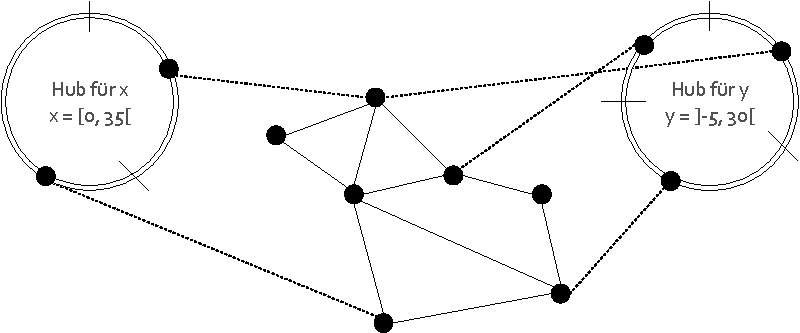
\includegraphics{grafics/mercury.pdf}}
\caption{Aufbau von Mercury}
\label{fig:mercury}
\end{figure}

\paragraph{Subscribe}
Eine Subscription $S$ ist ein Tupel aus Filterbedingungen über die Attribute, zum Beispiel $S := (5 < x <= 20; y = 15)$, sowie Kontaktinformationen des Knotens. Für jede Subscribtion wird das Attribut mit der größten Selektivität ausgewählt; im Beispiel ist dies Attribut $y$. $S$ wird nun an einen beliebigen Knoten im zuständigen Hub gesendet. Im Hub wird $S$ nun zu den Knoten weitergereicht, die den Wertebereich des Prädikats abdecken und dort in einer Liste gespeichert. Es ist möglich, dass eine Subscribtion -- je nach abgedecktem Wertebereich -- bei mehreren Knoten abgespeichert wird.

\paragraph{Unsubscribe}
Zur Abmeldung muss ein entsprechendes \enquote{Negativ}-Tupel zur Anmeldung an den selben Hub wie das Anmeldetupel gesendet werden. Am richtigen Knoten angekommen, wird der Listeneintrag entfernt.

\paragraph{Publish}
Eine Publikation $P$ ist ebenfalls ein Tupel mit bestimmten Werten der Attribute, wie zum Beispiel $P := (x = 10; y = 0)$. Im Unterschied zur Anmeldung wird eine Publikation an \emph{alle} Hubs gesendet und dort zum jeweils zuständigen Knoten weitergereicht. Dieser gleicht $P$ mit den gespeicherten Anmeldetupel ab und sendet $P$ an den zugehörigen Knoten.

Eine weitere Umsetzung eines filterbasierten Publish/Subscribe-Systems ist Mirinae. Hier wird der Wertebereich eines Attributes als Hyperwürfel dargestellt. Eine automatische Anpassung dieser Aufteilung ermöglicht eine schnelle Anpassung der Routingtabelle und damit einen kurzen Weg für die Nachrichten \cite{Choi2005Mirinae}.
